% DMA Session 4: CRISP-DM & Fallstudien
% 180-Minuten-Block (Vorlesung + Übung interwoven)

\documentclass[usenames,dvipsnames,10pt,aspectratio=169]{beamer}
\usepackage[T1]{fontenc}
\usepackage[utf8]{inputenc}
\usepackage{verbatim}

% Theme loaded via symlinks (update beamerTemplate/ for CD changes)
\usetheme{ims}

\usepackage{booktabs}
\usepackage{multicol}
\usepackage{listings}
\usepackage{xcolor}
\usepackage{graphicx}
\usepackage{tikz}
\usetikzlibrary{shapes.geometric, arrows.meta, positioning, calc, fit, backgrounds, matrix}

% ===== CLICKABLE AGENDA WITH PROGRESS INDICATOR =====
\usepackage{hyperref}
\hypersetup{colorlinks=false, pdfborder={0 0 0}}

% Phase counter for progress tracking
\newcounter{currentphase}
\setcounter{currentphase}{0}

% Clickable agenda item
\newcommand{\agendaitem}[3]{%
    \ifnum#1=#2
        \textcolor{IMSOrange}{$\blacktriangleright$ \textbf{\hyperlink{phase#2}{#3}}}%
    \else
        \textcolor{gray!70}{\phantom{$\blacktriangleright$} \hyperlink{phase#2}{#3}}%
    \fi\\[0.3em]%
}

% Progress dots for footline (clickable)
\newcommand{\progressdots}{%
    
\begin{tikzpicture}[baseline=-0.5ex]
        \foreach \i in {1,...,7} {
            \ifnum\value{currentphase}=\i
                \node[circle, fill=IMSOrange, minimum size=0.24cm, inner sep=0pt] at (\i*0.4,0) {\hyperlink{phase\i}{\phantom{oo}}};
            \else
                \ifnum\value{currentphase}>\i
                    \node[circle, fill=IMSBlue!60, minimum size=0.2cm, inner sep=0pt] at (\i*0.4,0) {\hyperlink{phase\i}{\phantom{oo}}};
                \else
                    \node[circle, draw=gray!50, minimum size=0.2cm, inner sep=0pt] at (\i*0.4,0) {\hyperlink{phase\i}{\phantom{oo}}};
                \fi
            \fi
        }
    \end{tikzpicture}%
}

% Add progress indicator to footline
\setbeamertemplate{footline}{%
    \leavevmode%
    \hbox{%
        \begin{beamercolorbox}[wd=.33\paperwidth,ht=2.5ex,dp=1ex,left]{author in head/foot}%
            \usebeamerfont{author in head/foot}\hspace*{2ex}\insertshortauthor
        \end{beamercolorbox}%
        \begin{beamercolorbox}[wd=.34\paperwidth,ht=2.5ex,dp=1ex,center]{title in head/foot}%
            \progressdots
        \end{beamercolorbox}%
        \begin{beamercolorbox}[wd=.33\paperwidth,ht=2.5ex,dp=1ex,right]{date in head/foot}%
            \usebeamerfont{date in head/foot}\insertframenumber{} / \inserttotalframenumber\hspace*{2ex}
        \end{beamercolorbox}%
    }%
    \vskip0pt%
}

% TikZ styles for diagrams
\tikzset{
    crispbox/.style={rectangle, rounded corners, minimum width=2.8cm, minimum height=1cm,
        text centered, align=center, draw=IMSBlue, fill=IMSBlue!15, font=\small\bfseries},
    crisparrow/.style={-{Stealth[length=2.5mm]}, thick, IMSOrange},
    sqlbox/.style={rectangle, rounded corners, minimum width=2.5cm, minimum height=0.8cm,
        text centered, draw=IMSBlue, fill=IMSBlue!15, font=\ttfamily\small},
    sqlarrow/.style={-{Stealth[length=2.5mm]}, thick, IMSOrange},
    databox/.style={rectangle, minimum width=1.2cm, minimum height=0.5cm,
        text centered, draw=gray, fill=gray!10, font=\small},
    alertbox/.style={rectangle, rounded corners, minimum width=2cm, minimum height=0.6cm,
        text centered, draw=red!70, fill=red!15, font=\small},
    goodbox/.style={rectangle, rounded corners, minimum width=2cm, minimum height=0.6cm,
        text centered, draw=green!60!black, fill=green!15, font=\small},
}

% SQL Listing Style
\lstdefinestyle{sql}{
    language=SQL,
    basicstyle=\ttfamily\footnotesize,
    keywordstyle=\color{IMSBlue}\bfseries,
    stringstyle=\color{IMSOrange},
    commentstyle=\color{gray}\itshape,
    showstringspaces=false,
    breaklines=true,
    frame=single,
    backgroundcolor=\color{gray!10},
    morekeywords={SERIAL, BOOLEAN, TEXT, COALESCE, SUBSTR, CAST, LOG10, FLOOR, ABS},
    literate={ü}{{\"u}}1 {ä}{{\"a}}1 {ö}{{\"o}}1 {Ü}{{\"U}}1 {Ä}{{\"A}}1 {Ö}{{\"O}}1 {ß}{{\ss}}1
}

\lstset{style=sql}

% Agenda reminder frame - argument is the current phase number
\newcommand{\showagenda}[1]{%
\setcounter{currentphase}{#1}%
\hypertarget{phase#1}{}%
\begin{frame}{Agenda}
\vfill
\begin{center}
\begin{minipage}{0.6\textwidth}
\large
\agendaitem{#1}{1}{1 ~ Rückblick \& CRISP-DM Einführung}
\agendaitem{#1}{2}{2 ~ Der CRISP-DM Prozess}
\agendaitem{#1}{3}{3 ~ Fallstudie I: Dr. Harold Shipman}
\agendaitem{#1}{4}{4 ~ SQL-Analyse des Shipman-Falls}
\agendaitem{#1}{5}{5 ~ Fallstudie II: Benford's Law}
\agendaitem{#1}{6}{6 ~ Betrugserkennung mit Ziffernanalyse}
\agendaitem{#1}{7}{7 ~ Zusammenfassung \& Ausblick}
\end{minipage}
\end{center}
\vfill
\end{frame}
}

%%%%%%%%%%%%%%%%%%%%%%%%%%%%%%%%%%%%%%%%%%%%%%%%%%%%%%%%%%%%%%%%%%%%%%%%%%%%%%%%%%%%%
\title[DMA 04]{Datenmanagement \& -analyse}
\subtitle{Vorlesung 4: CRISP-DM \& Fallstudien}
\date{Sommersemester 2026}
\author{Prof. Dr. Christoph M. Flath}
\institute{Data Driven Decisions Group, Universität Würzburg}
%%%%%%%%%%%%%%%%%%%%%%%%%%%%%%%%%%%%%%%%%%%%%%%%%%%%%%%%%%%%%%%%%%%%%%%%%%%%%%%%%%%%%

\begin{document}

\begin{frame}
\titlepage
\end{frame}

%%%%%%%%%%%%%%%%%%%%%%%%%%%%%%%%%%%%%%%%%%%%%%%%%%%%%%%%%%%%%%%%%%%%%%%%%%%%%%%%%%%%%
\section*{Agenda}
%%%%%%%%%%%%%%%%%%%%%%%%%%%%%%%%%%%%%%%%%%%%%%%%%%%%%%%%%%%%%%%%%%%%%%%%%%%%%%%%%%%%%

\begin{frame}{Agenda}
\vfill
\begin{center}
\begin{minipage}{0.6\textwidth}
\large
1 ~ Rückblick \& CRISP-DM Einführung\\[0.3em]
2 ~ Der CRISP-DM Prozess\\[0.3em]
3 ~ Fallstudie I: Dr. Harold Shipman\\[0.3em]
4 ~ SQL-Analyse des Shipman-Falls\\[0.3em]
5 ~ Fallstudie II: Benford's Law\\[0.3em]
6 ~ Betrugserkennung mit Ziffernanalyse\\[0.3em]
7 ~ Zusammenfassung \& Ausblick\\[0.3em]
\end{minipage}
\end{center}
\vfill
\begin{alertblock}{Lernziele}
Strukturierte Datenanalyseprozesse verstehen und auf reale Fallstudien anwenden.
\end{alertblock}
\end{frame}

%%%%%%%%%%%%%%%%%%%%%%%%%%%%%%%%%%%%%%%%%%%%%%%%%%%%%%%%%%%%%%%%%%%%%%%%%%%%%%%%%%%%%
\section{Phase 1: Rückblick \& CRISP-DM Einführung}
%%%%%%%%%%%%%%%%%%%%%%%%%%%%%%%%%%%%%%%%%%%%%%%%%%%%%%%%%%%%%%%%%%%%%%%%%%%%%%%%%%%%%

\showagenda{1}

\begin{frame}{Rückblick: Unser SQL-Werkzeugkasten}

\begin{tikzpicture}[node distance=0.3cm and 0.5cm]
    \node[sqlbox] (select) {SELECT};
    \node[sqlbox, right=of select] (from) {FROM};
    \node[sqlbox, right=of from] (where) {WHERE};
    \node[sqlbox, right=of where] (order) {ORDER BY};

    \node[sqlbox, below=0.8cm of select] (agg) {COUNT/SUM/AVG};
    \node[sqlbox, right=of agg] (group) {GROUP BY};
    \node[sqlbox, right=of group] (having) {HAVING};
    \node[sqlbox, right=of having] (distinct) {DISTINCT};

    \draw[sqlarrow] (select) -- (from);
    \draw[sqlarrow] (from) -- (where);
    \draw[sqlarrow] (where) -- (order);

    \draw[sqlarrow] (agg) -- (group);
    \draw[sqlarrow] (group) -- (having);
\end{tikzpicture}

\vspace{0.5cm}

\textbf{Bisher gelernt:}
\begin{itemize}
    \item Daten abfragen, filtern und sortieren
    \item Aggregieren und gruppieren
    \item NULL-Werte behandeln
\end{itemize}

\textbf{Heute:} Diese Werkzeuge systematisch einsetzen!

\end{frame}

\begin{frame}{Von der Technik zur Methodik}

\begin{columns}
\begin{column}{0.5\textwidth}
\textbf{Bisher: Einzelne Abfragen}
\begin{itemize}
    \item ``Zeige alle Spieler''
    \item ``Wie viele Tore?''
    \item ``Gruppiere nach Position''
\end{itemize}

\vspace{0.5cm}

$\Rightarrow$ Isolierte technische Übungen
\end{column}

\begin{column}{0.5\textwidth}
\textbf{Heute: Strukturierte Analyse}
\begin{itemize}
    \item Geschäftsproblem verstehen
    \item Daten systematisch erkunden
    \item Hypothesen prüfen
    \item Erkenntnisse kommunizieren
\end{itemize}

\vspace{0.3cm}

$\Rightarrow$ Professionelle Datenanalyse
\end{column}
\end{columns}

\vspace{0.5cm}

\begin{exampleblock}{Kernfrage}
Wie gehen professionelle Datenanalysten systematisch vor?
\end{exampleblock}

\end{frame}

\begin{frame}{Warum brauchen wir einen Prozess?}

\begin{columns}
\begin{column}{0.5\textwidth}
\textbf{Ohne Struktur:}
\begin{itemize}
    \item Ad-hoc Abfragen
    \item Wichtige Fragen übersehen
    \item Ergebnisse nicht reproduzierbar
    \item Fehlinterpretationen
    \item Zeit verschwendet
\end{itemize}
\end{column}

\begin{column}{0.5\textwidth}
\textbf{Mit Struktur:}
\begin{itemize}
    \item Klare Zielsetzung
    \item Systematische Exploration
    \item Dokumentierte Schritte
    \item Validierte Ergebnisse
    \item Effiziente Arbeit
\end{itemize}
\end{column}
\end{columns}

\vspace{0.5cm}

\begin{alertblock}{Realität}
80\% der Analysezeit geht für Datenvorbereitung drauf -- \\
ein guter Prozess hilft, diese Zeit sinnvoll zu nutzen.
\end{alertblock}

\end{frame}

%%%%%%%%%%%%%%%%%%%%%%%%%%%%%%%%%%%%%%%%%%%%%%%%%%%%%%%%%%%%%%%%%%%%%%%%%%%%%%%%%%%%%
\section{Phase 2: Der CRISP-DM Prozess}
%%%%%%%%%%%%%%%%%%%%%%%%%%%%%%%%%%%%%%%%%%%%%%%%%%%%%%%%%%%%%%%%%%%%%%%%%%%%%%%%%%%%%

\showagenda{2}

\begin{frame}{CRISP-DM: Cross-Industry Standard Process}

\begin{center}
\begin{tikzpicture}[scale=0.9]
    % Circular arrangement of phases
    \node[crispbox] (bu) at (90:3cm) {Business\\Understanding};
    \node[crispbox] (du) at (30:3cm) {Data\\Understanding};
    \node[crispbox] (dp) at (-30:3cm) {Data\\Preparation};
    \node[crispbox] (mo) at (-90:3cm) {Modeling};
    \node[crispbox] (ev) at (-150:3cm) {Evaluation};
    \node[crispbox] (de) at (150:3cm) {Deployment};

    % Center
    \node[draw=IMSOrange, fill=IMSOrange!20, circle, minimum size=1.5cm, font=\small\bfseries] (data) at (0,0) {Data};

    % Arrows (clockwise)
    \draw[crisparrow, bend left=15] (bu) to (du);
    \draw[crisparrow, bend left=15] (du) to (dp);
    \draw[crisparrow, bend left=15] (dp) to (mo);
    \draw[crisparrow, bend left=15] (mo) to (ev);
    \draw[crisparrow, bend left=15] (ev) to (de);
    \draw[crisparrow, bend left=15] (de) to (bu);

    % Back arrows (iteration) - using bend right for counter-clockwise flow
    \draw[crisparrow, dashed, bend right=25] (du) to (bu);
    \draw[crisparrow, dashed, bend left=40] (ev.north west) to (bu.south west);
\end{tikzpicture}
\end{center}

\vspace{0.3cm}

\textbf{Industrie-Standard} seit 1996 -- entwickelt von IBM, NCR, SPSS, Daimler

\end{frame}

\begin{frame}{Phase 1: Business Understanding}

\begin{columns}
\begin{column}{0.6\textwidth}
\textbf{Kernfragen:}
\begin{itemize}
    \item Was ist das Geschäftsziel?
    \item Welches Problem soll gelöst werden?
    \item Wie wird Erfolg gemessen?
    \item Wer sind die Stakeholder?
\end{itemize}

\vspace{0.5cm}

\textbf{Output:}
\begin{itemize}
    \item Klare Problemdefinition
    \item Erfolgskriterien
    \item Projektplan
\end{itemize}
\end{column}

\begin{column}{0.4\textwidth}
\begin{exampleblock}{Beispiel: Shipman}
``Gibt es Ärzte mit ungewöhnlich\\
hohen Sterberaten?''

\vspace{0.3cm}

$\Rightarrow$ Anomalie-Erkennung\\
$\Rightarrow$ Patientensicherheit
\end{exampleblock}
\end{column}
\end{columns}

\end{frame}

\begin{frame}{Phase 2: Data Understanding}

\begin{columns}
\begin{column}{0.6\textwidth}
\textbf{Aktivitäten:}
\begin{itemize}
    \item Daten sammeln
    \item Daten beschreiben (Struktur, Umfang)
    \item Daten erkunden (Verteilungen, Muster)
    \item Datenqualität prüfen
\end{itemize}

\vspace{0.5cm}

\textbf{SQL-Werkzeuge:}
\begin{itemize}
    \item \texttt{SELECT *} -- Struktur verstehen
    \item \texttt{COUNT}, \texttt{DISTINCT} -- Umfang
    \item \texttt{MIN}, \texttt{MAX}, \texttt{AVG} -- Verteilungen
    \item \texttt{IS NULL} -- Datenqualität
\end{itemize}
\end{column}

\begin{column}{0.4\textwidth}
\begin{alertblock}{Häufige Probleme}
\begin{itemize}
    \item Fehlende Werte
    \item Inkonsistente Formate
    \item Duplikate
    \item Ausreißer
\end{itemize}
\end{alertblock}
\end{column}
\end{columns}

\end{frame}

\begin{frame}{Phase 3: Data Preparation}

\textbf{Die arbeitsintensivste Phase!}

\vspace{0.5cm}

\begin{columns}
\begin{column}{0.5\textwidth}
\textbf{Typische Aufgaben:}
\begin{itemize}
    \item Daten bereinigen
    \item Fehlende Werte behandeln
    \item Variablen transformieren
    \item Daten zusammenführen
    \item Stichproben ziehen
\end{itemize}
\end{column}

\begin{column}{0.5\textwidth}
\textbf{SQL-Beispiele:}
\begin{itemize}
    \item \texttt{COALESCE} für NULL
    \item \texttt{CAST} für Typumwandlung
    \item \texttt{SUBSTR} für Textextraktion
    \item \texttt{JOIN} für Verknüpfungen
    \item \texttt{WHERE} für Filter
\end{itemize}
\end{column}
\end{columns}

\vspace{0.5cm}

\begin{exampleblock}{Faustregel}
Plane 60-80\% der Projektzeit für Datenvorbereitung ein!
\end{exampleblock}

\end{frame}

\begin{frame}{Datenqualität: Die 6 Dimensionen}

\begin{center}
\begin{tikzpicture}[scale=0.75]
    % Six boxes arranged in 2 rows - using relative positioning
    \node[crispbox, minimum width=3.8cm] (v) at (0,2) {\textbf{Vollständigkeit}\\Keine fehlenden Werte};
    \node[crispbox, minimum width=3.8cm] (k) at (4.8,2) {\textbf{Korrektheit}\\Werte sind richtig};
    \node[crispbox, minimum width=3.8cm] (ko) at (9.6,2) {\textbf{Konsistenz}\\Keine Widersprüche};

    \node[crispbox, minimum width=3.8cm] (a) at (0,-0.5) {\textbf{Aktualität}\\Daten sind aktuell};
    \node[crispbox, minimum width=3.8cm] (e) at (4.8,-0.5) {\textbf{Eindeutigkeit}\\Keine Duplikate};
    \node[crispbox, minimum width=3.8cm] (g) at (9.6,-0.5) {\textbf{Gültigkeit}\\Format/Wertebereich OK};
\end{tikzpicture}
\end{center}

\vspace{0.5cm}

\begin{alertblock}{``Garbage In, Garbage Out''}
Die beste Analyse ist wertlos, wenn die Eingabedaten schlecht sind.\\
Datenqualität ist keine Option, sondern Voraussetzung für jeden Analyseerfolg!
\end{alertblock}

\end{frame}

\begin{frame}{Phase 4-6: Modeling, Evaluation, Deployment}

\begin{columns}
\begin{column}{0.33\textwidth}
\textbf{Modeling:}
\begin{itemize}
    \item Technik wählen
    \item Modell bauen
    \item Parameter optimieren
\end{itemize}

\vspace{0.3cm}

\textit{(Oft mit ML-Tools,\\
aber auch SQL-Analysen)}
\end{column}

\begin{column}{0.33\textwidth}
\textbf{Evaluation:}
\begin{itemize}
    \item Ergebnisse prüfen
    \item Geschäftsziele erreicht?
    \item Nächste Schritte?
\end{itemize}

\vspace{0.3cm}

\textit{(Zurück zu Phase 1\\
wenn nötig)}
\end{column}

\begin{column}{0.33\textwidth}
\textbf{Deployment:}
\begin{itemize}
    \item Lösung einsetzen
    \item Dokumentieren
    \item Monitoring planen
\end{itemize}

\vspace{0.3cm}

\textit{(Dashboards, Reports,\\
automatisierte Abfragen)}
\end{column}
\end{columns}

\vspace{0.5cm}

\begin{alertblock}{Wichtig}
CRISP-DM ist iterativ -- man springt oft zwischen Phasen!
\end{alertblock}

\end{frame}

\begin{frame}{Vorhersage: CRISP-DM Phasen}

\textbf{Ordne die Aktivitäten den CRISP-DM Phasen zu:}

\vspace{0.5cm}

\begin{tabular}{p{6cm}l}
\toprule
\textbf{Aktivität} & \textbf{Phase?} \\
\midrule
``Wir wollen Kundenabwanderung reduzieren'' & ??? \\
NULL-Werte mit Durchschnitt ersetzen & ??? \\
COUNT und AVG über alle Spalten & ??? \\
Dashboard für Management erstellen & ??? \\
Modell mit Testdaten validieren & ??? \\
\bottomrule
\end{tabular}

\vspace{0.5cm}

\pause

\textbf{Lösung:} Business Understanding, Data Preparation, Data Understanding, Deployment, Evaluation

\end{frame}

%%%%%%%%%%%%%%%%%%%%%%%%%%%%%%%%%%%%%%%%%%%%%%%%%%%%%%%%%%%%%%%%%%%%%%%%%%%%%%%%%%%%%
\section{Phase 3: Fallstudie I -- Dr. Harold Shipman}
%%%%%%%%%%%%%%%%%%%%%%%%%%%%%%%%%%%%%%%%%%%%%%%%%%%%%%%%%%%%%%%%%%%%%%%%%%%%%%%%%%%%%

\showagenda{3}

\begin{frame}{Der Fall Harold Shipman}

\begin{columns}
\begin{column}{0.6\textwidth}
\textbf{Hintergrund:}
\begin{itemize}
    \item Britischer Hausarzt (1946-2004)
    \item Praktizierte in Hyde, Greater Manchester
    \item Über 23 Jahre als Arzt tätig
    \item Beliebter und respektierter Mediziner
\end{itemize}

\vspace{0.5cm}

\textbf{Die erschreckende Wahrheit:}
\begin{itemize}
    \item Mind. 215 Patienten ermordet
    \item Meist ältere Frauen
    \item Tötung durch Morphin-Überdosis
    \item Produktivster Serienmörder der UK-Geschichte
\end{itemize}
\end{column}

\begin{column}{0.4\textwidth}
\begin{alertblock}{Kernfrage}
Hätte Datenanalyse die Morde früher aufdecken können?
\end{alertblock}

\vspace{0.3cm}

\begin{exampleblock}{Spoiler}
Ja -- die Muster waren in den Daten sichtbar!
\end{exampleblock}
\end{column}
\end{columns}

\end{frame}

\begin{frame}{Wie wurde Shipman entdeckt?}

\begin{columns}
\begin{column}{0.6\textwidth}
\textbf{1998: Der letzte Mord}
\begin{itemize}
    \item Kathleen Grundy (81) stirbt
    \item Shipman fälscht ihr Testament
    \item Tochter (Anwältin!) wird misstrauisch
    \item Exhumierung $\Rightarrow$ Morphin nachgewiesen
\end{itemize}

\vspace{0.5cm}

\textbf{Untersuchung danach:}
\begin{itemize}
    \item Statistische Analyse aller Todesfälle
    \item Shipmans Raten \textbf{extrem} auffällig
    \item Muster über Jahrzehnte erkennbar
\end{itemize}
\end{column}

\begin{column}{0.4\textwidth}
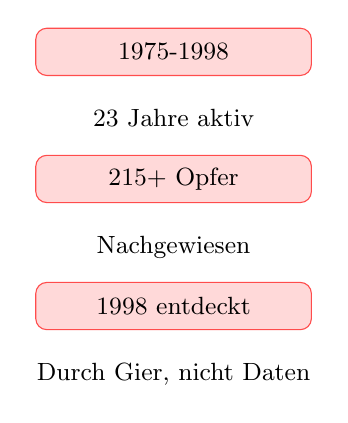
\begin{tikzpicture}
    \node[alertbox, minimum width=3.5cm] (a) {1975-1998};
    \node[below=0.3cm of a, font=\small] {23 Jahre aktiv};

    \node[alertbox, minimum width=3.5cm, below=1cm of a] (b) {215+ Opfer};
    \node[below=0.3cm of b, font=\small] {Nachgewiesen};

    \node[alertbox, minimum width=3.5cm, below=1cm of b] (c) {1998 entdeckt};
    \node[below=0.3cm of c, font=\small] {Durch Gier, nicht Daten};
\end{tikzpicture}
\end{column}
\end{columns}

\end{frame}

\begin{frame}{CRISP-DM angewandt: Business Understanding}

\textbf{Geschäftsproblem:}
\begin{itemize}
    \item Patientensicherheit gewährleisten
    \item Ungewöhnliche Sterbemuster erkennen
    \item Ärzte mit Anomalien identifizieren
\end{itemize}

\vspace{0.5cm}

\textbf{Analysefragen:}
\begin{enumerate}
    \item Wie viele Patienten sterben pro Arzt?
    \item Gibt es Ärzte mit überdurchschnittlich vielen Todesfällen?
    \item Zu welchen Uhrzeiten sterben die Patienten?
    \item Gibt es Muster bei Alter oder Geschlecht der Verstorbenen?
\end{enumerate}

\vspace{0.3cm}

\begin{exampleblock}{Erfolgskriterium}
Identifikation von Ärzten, deren Sterberaten signifikant vom Durchschnitt abweichen.
\end{exampleblock}

\end{frame}

\begin{frame}{Die Daten}

\textbf{Verfügbare Informationen (vereinfacht):}

\vspace{0.3cm}

\begin{tabular}{lll}
\toprule
\textbf{Tabelle} & \textbf{Spalten} & \textbf{Beschreibung} \\
\midrule
\texttt{deaths} & patient\_id, doctor\_id, & Todesfälle \\
 & death\_date, death\_time, & \\
 & age, gender, cause & \\
\midrule
\texttt{doctors} & doctor\_id, name, & Ärzte \\
 & practice, start\_year & \\
\midrule
\texttt{patients} & patient\_id, doctor\_id, & Patientenstamm \\
 & registration\_date & \\
\bottomrule
\end{tabular}

\vspace{0.5cm}

\textbf{Frage:} Welche SQL-Abfragen würden Sie stellen?

\end{frame}

%%%%%%%%%%%%%%%%%%%%%%%%%%%%%%%%%%%%%%%%%%%%%%%%%%%%%%%%%%%%%%%%%%%%%%%%%%%%%%%%%%%%%
\section{Phase 4: SQL-Analyse des Shipman-Falls}
%%%%%%%%%%%%%%%%%%%%%%%%%%%%%%%%%%%%%%%%%%%%%%%%%%%%%%%%%%%%%%%%%%%%%%%%%%%%%%%%%%%%%

\showagenda{4}

\begin{frame}[fragile]{Analyse 1: Todesfälle pro Arzt}

\textbf{Data Understanding:} Wie verteilen sich die Todesfälle?

\begin{lstlisting}
SELECT
    d.name AS arzt,
    COUNT(*) AS todesfaelle
FROM deaths de
JOIN doctors d ON de.doctor_id = d.doctor_id
GROUP BY d.doctor_id, d.name
ORDER BY todesfaelle DESC;
\end{lstlisting}

\vspace{0.3cm}

\textbf{Erwartetes Ergebnis:}

\begin{tabular}{lr}
\toprule
\textbf{arzt} & \textbf{todesfaelle} \\
\midrule
Dr. Shipman & 297 \\
Dr. Smith & 45 \\
Dr. Jones & 42 \\
... & ... \\
\bottomrule
\end{tabular}

$\Rightarrow$ \textbf{Shipman: 6-7x mehr als Kollegen!}

\end{frame}

\begin{frame}[fragile]{Analyse 2: Sterbezeit-Verteilung}

\textbf{Hypothese:} Natürliche Todesfälle verteilen sich über den Tag

\begin{lstlisting}
SELECT
    doctor_id,
    CASE
        WHEN death_time BETWEEN '09:00' AND '17:00'
        THEN 'Praxiszeit'
        ELSE 'Ausserhalb'
    END AS zeitraum,
    COUNT(*) AS anzahl
FROM deaths
GROUP BY doctor_id, zeitraum;
\end{lstlisting}

\vspace{0.3cm}

\begin{columns}
\begin{column}{0.5\textwidth}
\textbf{Normale Ärzte:}\\
Praxiszeit: 35\%\\
Außerhalb: 65\%
\end{column}

\begin{column}{0.5\textwidth}
\textbf{Shipman:}\\
Praxiszeit: \textcolor{red}{\textbf{83\%}}\\
Außerhalb: 17\%
\end{column}
\end{columns}

\end{frame}

\begin{frame}[fragile]{Analyse 3: Geschlechterverteilung}

\begin{lstlisting}
SELECT
    d.name AS arzt,
    gender AS geschlecht,
    COUNT(*) AS anzahl,
    ROUND(COUNT(*) * 100.0 / SUM(COUNT(*)) OVER
        (PARTITION BY d.name), 1) AS prozent
FROM deaths de
JOIN doctors d ON de.doctor_id = d.doctor_id
GROUP BY d.name, gender;
\end{lstlisting}

\vspace{0.3cm}

\begin{columns}
\begin{column}{0.5\textwidth}
\textbf{Normale Verteilung:}\\
Männlich: $\approx$ 48\%\\
Weiblich: $\approx$ 52\%
\end{column}

\begin{column}{0.5\textwidth}
\textbf{Shipman:}\\
Männlich: 19\%\\
Weiblich: \textcolor{red}{\textbf{81\%}}
\end{column}
\end{columns}

\vspace{0.5cm}

$\Rightarrow$ Starke Abweichung bei Geschlechterverteilung!

\end{frame}

\begin{frame}[fragile]{Analyse 4: Altersverteilung}

\begin{lstlisting}
SELECT
    d.name AS arzt,
    AVG(de.age) AS durchschnittsalter,
    MIN(de.age) AS juengstes_opfer,
    MAX(de.age) AS aeltestes_opfer
FROM deaths de
JOIN doctors d ON de.doctor_id = d.doctor_id
GROUP BY d.name;
\end{lstlisting}

\vspace{0.5cm}

\textbf{Auffälligkeit:}
\begin{itemize}
    \item Shipmans Patienten: Durchschnitt 77 Jahre
    \item Aber: Auch ``gesunde'' 65-Jährige
    \item Typisch für Mord: Opferprofil ist konsistent
\end{itemize}

\end{frame}

\begin{frame}[fragile]{Übung: Weitere Anomalien finden}

\textbf{Aufgabe:} Schreibe eine SQL-Abfrage, die zeigt:

\begin{enumerate}
    \item Wie viele Patienten pro Arzt in den \textbf{ersten 6 Monaten} nach Registrierung sterben
    \item Gruppiert nach Arzt
    \item Sortiert nach Anzahl (absteigend)
\end{enumerate}

\vspace{0.5cm}

\textbf{Hinweis:} Neue Patienten sollten eigentlich nicht so schnell sterben...

\vspace{0.5cm}

\pause

\begin{lstlisting}
SELECT d.name, COUNT(*) AS fruehe_tode
FROM deaths de
JOIN doctors d ON de.doctor_id = d.doctor_id
JOIN patients p ON de.patient_id = p.patient_id
WHERE de.death_date <= p.registration_date + 180
GROUP BY d.name
ORDER BY fruehe_tode DESC;
\end{lstlisting}

\end{frame}

\begin{frame}{Lehren aus dem Shipman-Fall}

\begin{columns}
\begin{column}{0.5\textwidth}
\textbf{Was die Daten zeigten:}
\begin{itemize}
    \item Extreme Sterberate
    \item Ungewöhnliche Uhrzeiten
    \item Bias bei Geschlecht/Alter
    \item Muster über Jahre konsistent
\end{itemize}

\vspace{0.3cm}

\textbf{Warum wurde es übersehen?}
\begin{itemize}
    \item Keine systematische Analyse
    \item Daten nicht verknüpft
    \item Kein Monitoring-System
\end{itemize}
\end{column}

\begin{column}{0.5\textwidth}
\begin{alertblock}{Konsequenz}
UK führte nach Shipman systematisches Mortality Monitoring ein.

\vspace{0.3cm}

SQL-Abfragen wie unsere laufen jetzt \textbf{automatisch}!
\end{alertblock}

\vspace{0.3cm}

\begin{exampleblock}{CRISP-DM Lektion}
Data Understanding hätte das Problem aufgedeckt -- wenn jemand hingeschaut hätte.
\end{exampleblock}
\end{column}
\end{columns}

\end{frame}

\begin{frame}{Pause}

\begin{center}
\Large
\textbf{10 Minuten Pause}

\vspace{1cm}

\normalsize
Nach der Pause:\\
Benford's Law -- Wie Zahlen Betrug verraten
\end{center}

\end{frame}

%%%%%%%%%%%%%%%%%%%%%%%%%%%%%%%%%%%%%%%%%%%%%%%%%%%%%%%%%%%%%%%%%%%%%%%%%%%%%%%%%%%%%
\section{Phase 5: Fallstudie II -- Benford's Law}
%%%%%%%%%%%%%%%%%%%%%%%%%%%%%%%%%%%%%%%%%%%%%%%%%%%%%%%%%%%%%%%%%%%%%%%%%%%%%%%%%%%%%

\showagenda{5}

\begin{frame}{Benford's Law: Eine überraschende Entdeckung}

\begin{columns}
\begin{column}{0.55\textwidth}
\textbf{Die Beobachtung (1881):}

Simon Newcomb bemerkte, dass Logarithmentafeln vorne abgegriffener waren als hinten.

\vspace{0.3cm}

\textbf{Frank Benford (1938):}

Analysierte 20.000+ Zahlen aus verschiedensten Quellen:
\begin{itemize}
    \item Flusslängen
    \item Bevölkerungszahlen
    \item Physikalische Konstanten
    \item Zeitungsartikel
\end{itemize}
\end{column}

\begin{column}{0.45\textwidth}
\begin{tikzpicture}[scale=0.7]
    % Bar chart - scale: 1 unit = 10%
    \draw[->] (0,0) -- (5,0) node[right] {Ziffer};
    \draw[->] (0,0) -- (0,3.5) node[above] {\%};

    % Y-axis tick marks
    \draw (0,1) -- (-0.1,1) node[left, font=\tiny] {10};
    \draw (0,2) -- (-0.1,2) node[left, font=\tiny] {20};
    \draw (0,3) -- (-0.1,3) node[left, font=\tiny] {30};

    % Bars (Benford distribution) - height = percentage/10
    \fill[IMSBlue!70] (0.2,0) rectangle (0.6,3.01);  % 1: 30.1%
    \fill[IMSBlue!70] (0.7,0) rectangle (1.1,1.76);  % 2: 17.6%
    \fill[IMSBlue!70] (1.2,0) rectangle (1.6,1.25);  % 3: 12.5%
    \fill[IMSBlue!70] (1.7,0) rectangle (2.1,0.97);  % 4: 9.7%
    \fill[IMSBlue!70] (2.2,0) rectangle (2.6,0.79);  % 5: 7.9%
    \fill[IMSBlue!70] (2.7,0) rectangle (3.1,0.67);  % 6: 6.7%
    \fill[IMSBlue!70] (3.2,0) rectangle (3.6,0.58);  % 7: 5.8%
    \fill[IMSBlue!70] (3.7,0) rectangle (4.1,0.51);  % 8: 5.1%
    \fill[IMSBlue!70] (4.2,0) rectangle (4.6,0.46);  % 9: 4.6%

    % X-axis digit labels
    \foreach \x/\d in {0.4/1, 0.9/2, 1.4/3, 1.9/4, 2.4/5, 2.9/6, 3.4/7, 3.9/8, 4.4/9} {
        \node[below, font=\tiny] at (\x,0) {\d};
    }

    % Percentage labels on top of bars
    \node[above, font=\tiny] at (0.4,3.01) {30\%};
    \node[above, font=\tiny] at (0.9,1.76) {18\%};
\end{tikzpicture}

\vspace{0.3cm}

\textbf{Erwartung:} Jede Ziffer $\approx$ 11\%\\
\textbf{Realität:} 1 kommt 6x häufiger vor als 9!
\end{column}
\end{columns}

\end{frame}

\begin{frame}{Die Benford-Verteilung}

\textbf{Mathematische Formel:}

$$P(d) = \log_{10}\left(1 + \frac{1}{d}\right)$$

\vspace{0.3cm}

\begin{tabular}{c|ccccccccc}
\toprule
\textbf{Erste Ziffer} & 1 & 2 & 3 & 4 & 5 & 6 & 7 & 8 & 9 \\
\midrule
\textbf{Erwartete \%} & 30.1 & 17.6 & 12.5 & 9.7 & 7.9 & 6.7 & 5.8 & 5.1 & 4.6 \\
\bottomrule
\end{tabular}

\vspace{0.5cm}

\textbf{Warum funktioniert das?}
\begin{itemize}
    \item Natürliche Daten wachsen oft \textbf{multiplikativ} (exponentiell)
    \item Um von 1xx auf 2xx zu kommen: +100\% Wachstum nötig
    \item Um von 8xx auf 9xx zu kommen: nur +12.5\% Wachstum nötig
    \item $\Rightarrow$ Zahlen ``verbringen mehr Zeit'' mit führender 1
\end{itemize}

\end{frame}

\begin{frame}{Wann gilt Benford's Law?}

\begin{columns}
\begin{column}{0.5\textwidth}
\textbf{Funktioniert gut bei:}
\begin{itemize}
    \item Finanzdaten (Rechnungen, Ausgaben)
    \item Bevölkerungszahlen
    \item Aktienkurse
    \item Naturwissenschaftliche Messungen
    \item Wahlergebnisse (Stimmen pro Bezirk)
\end{itemize}

\vspace{0.3cm}

$\Rightarrow$ Daten, die über mehrere Größenordnungen variieren
\end{column}

\begin{column}{0.5\textwidth}
\textbf{Funktioniert NICHT bei:}
\begin{itemize}
    \item Telefonnummern (feste Struktur)
    \item Postleitzahlen (zugewiesen)
    \item Preise (psychologisch: 9,99€)
    \item Körpergrößen (enger Bereich)
    \item Zufallszahlen
\end{itemize}

\vspace{0.3cm}

$\Rightarrow$ Daten mit eingeschränktem Wertebereich oder menschlichem Design
\end{column}
\end{columns}

\end{frame}

\begin{frame}{Benford zur Betrugserkennung}

\textbf{Die Idee:}

Menschen, die Zahlen \textbf{erfinden}, verteilen Ziffern oft gleichmäßig -- oder vermeiden ``auffällige'' Muster.

\vspace{0.5cm}

\begin{columns}
\begin{column}{0.5\textwidth}
\textbf{Echte Spesenabrechnungen:}
\begin{itemize}
    \item Folgen Benford
    \item Viele kleine Beträge
    \item Natürliche Variation
\end{itemize}
\end{column}

\begin{column}{0.5\textwidth}
\textbf{Gefälschte Abrechnungen:}
\begin{itemize}
    \item Zu viele 5er und 6er
    \item ``Runde'' Beträge
    \item Künstliche Gleichverteilung
\end{itemize}
\end{column}
\end{columns}

\vspace{0.5cm}

\begin{alertblock}{Anwendungen}
\begin{itemize}
    \item Steuerbetrug (IRS nutzt Benford!)
    \item Bilanzbetrug (Enron wurde damit analysiert)
    \item Wissenschaftlicher Betrug (gefälschte Daten)
    \item Wahlbetrug
\end{itemize}
\end{alertblock}

\end{frame}

\begin{frame}{Vorhersage: Benford oder nicht?}

\textbf{Welche Datensätze folgen Benford's Law?}

\vspace{0.5cm}

\begin{tabular}{lc}
\toprule
\textbf{Datensatz} & \textbf{Benford?} \\
\midrule
Umsätze aller DAX-Unternehmen & ??? \\
Hausnummern in Würzburg & ??? \\
Einwohnerzahlen aller Länder & ??? \\
Instagram-Follower von Influencern & ??? \\
Lottozahlen der letzten 10 Jahre & ??? \\
\bottomrule
\end{tabular}

\vspace{0.5cm}

\pause

\textbf{Lösungen:} Ja, Nein (zugewiesen), Ja, Ja (wachsen exponentiell), Nein (Zufall im festen Bereich)

\end{frame}

%%%%%%%%%%%%%%%%%%%%%%%%%%%%%%%%%%%%%%%%%%%%%%%%%%%%%%%%%%%%%%%%%%%%%%%%%%%%%%%%%%%%%
\section{Phase 6: Betrugserkennung mit Ziffernanalyse}
%%%%%%%%%%%%%%%%%%%%%%%%%%%%%%%%%%%%%%%%%%%%%%%%%%%%%%%%%%%%%%%%%%%%%%%%%%%%%%%%%%%%%

\showagenda{6}

\begin{frame}[fragile]{SQL: Erste Ziffer extrahieren}

\textbf{Schritt 1:} Die erste Ziffer jeder Zahl ermitteln

\begin{lstlisting}
-- Variante 1: String-Manipulation
SELECT
    betrag,
    CAST(SUBSTR(CAST(ABS(betrag) AS TEXT), 1, 1) AS INTEGER)
        AS erste_ziffer
FROM rechnungen
WHERE betrag > 0;
\end{lstlisting}

\begin{lstlisting}
-- Variante 2: Mathematisch (eleganter)
SELECT
    betrag,
    CAST(ABS(betrag) / POWER(10, FLOOR(LOG10(ABS(betrag))))
        AS INTEGER) AS erste_ziffer
FROM rechnungen
WHERE betrag > 0;
\end{lstlisting}

\end{frame}

\begin{frame}[fragile]{SQL: Ziffernverteilung berechnen}

\begin{lstlisting}
SELECT
    CAST(SUBSTR(CAST(betrag AS TEXT), 1, 1) AS INTEGER)
        AS erste_ziffer,
    COUNT(*) AS anzahl,
    ROUND(COUNT(*) * 100.0 / (SELECT COUNT(*) FROM rechnungen
        WHERE betrag > 0), 1) AS prozent
FROM rechnungen
WHERE betrag > 0
GROUP BY erste_ziffer
ORDER BY erste_ziffer;
\end{lstlisting}

\vspace{0.3cm}

\textbf{Beispiel-Output:}

\begin{tabular}{rrr}
\toprule
erste\_ziffer & anzahl & prozent \\
\midrule
1 & 3012 & 30.1 \\
2 & 1761 & 17.6 \\
... & ... & ... \\
\bottomrule
\end{tabular}

\end{frame}

\begin{frame}[fragile]{Abweichung von Benford messen}

\begin{lstlisting}
WITH ziffern AS (
    SELECT CAST(SUBSTR(CAST(betrag AS TEXT), 1, 1) AS INT) AS d,
           COUNT(*) AS n
    FROM rechnungen WHERE betrag > 0
    GROUP BY d
),
benford AS (
    SELECT 1 AS d, 0.301 AS erwartet UNION ALL
    SELECT 2, 0.176 UNION ALL
    SELECT 3, 0.125 UNION ALL
    -- ... weitere Ziffern
)
SELECT
    z.d AS ziffer,
    z.n AS beobachtet,
    ROUND(b.erwartet * (SELECT SUM(n) FROM ziffern), 0) AS erwartet,
    ROUND(ABS(z.n - b.erwartet * (SELECT SUM(n) FROM ziffern)), 0)
        AS abweichung
FROM ziffern z
JOIN benford b ON z.d = b.d;
\end{lstlisting}

\end{frame}

\begin{frame}[fragile]{Visualisierung: Erwartet vs. Beobachtet}

\textbf{Streudiagramm} zeigt Abweichung von Benford auf einen Blick:

\begin{columns}
\begin{column}{0.5\textwidth}
\begin{lstlisting}[language=Python, morekeywords={px}]
px.scatter(vergleich,
           x="erwartet_pct",
           y="beobachtet_pct",
           text="ziffer",
           title="Benford-Check")
\end{lstlisting}

\vspace{0.3cm}

\textbf{Interpretation:}
\begin{itemize}
    \item Punkte auf Diagonale = OK
    \item Abweichung = Verdacht
    \item Je weiter weg, desto auffälliger
\end{itemize}
\end{column}

\begin{column}{0.5\textwidth}
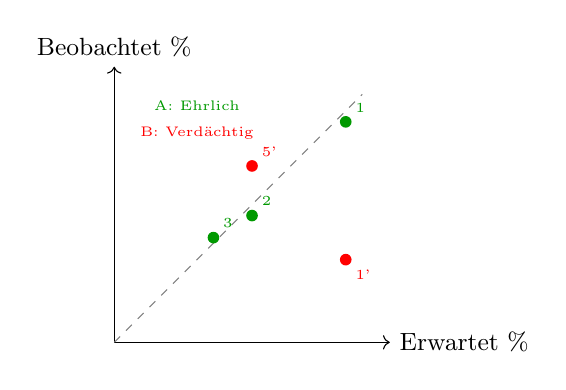
\begin{tikzpicture}[scale=0.7]
    \draw[->] (0,0) -- (5,0) node[right, font=\small] {Erwartet \%};
    \draw[->] (0,0) -- (0,5) node[above, font=\small] {Beobachtet \%};
    \draw[dashed, gray] (0,0) -- (4.5,4.5);
    % Good data points (near diagonal) - Employee A
    \fill[green!60!black] (4.2,4.0) circle (3pt) node[above right, font=\tiny] {1};
    \fill[green!60!black] (2.5,2.3) circle (3pt) node[above right, font=\tiny] {2};
    \fill[green!60!black] (1.8,1.9) circle (3pt) node[above right, font=\tiny] {3};
    % Bad data points (off diagonal) - Employee B
    \fill[red] (4.2,1.5) circle (3pt) node[below right, font=\tiny] {1'};
    \fill[red] (2.5,3.2) circle (3pt) node[above right, font=\tiny] {5'};
    % Legend
    \node[font=\tiny, green!60!black] at (1.5,4.3) {A: Ehrlich};
    \node[font=\tiny, red] at (1.5,3.8) {B: Verdächtig};
\end{tikzpicture}
\end{column}
\end{columns}

\end{frame}

\begin{frame}{Fallbeispiel: Spesenbetrug}

\textbf{Szenario:}

Ein Mitarbeiter reicht monatlich Spesenabrechnungen ein. Die Buchhaltung wird misstrauisch.

\vspace{0.5cm}

\begin{columns}
\begin{column}{0.5\textwidth}
\textbf{Mitarbeiter A (ehrlich):}

\begin{tabular}{cr}
\toprule
Ziffer & Anteil \\
\midrule
1 & 29.5\% \\
2 & 18.2\% \\
3 & 11.8\% \\
... & ... \\
\bottomrule
\end{tabular}

$\checkmark$ Passt zu Benford
\end{column}

\begin{column}{0.5\textwidth}
\textbf{Mitarbeiter B (verdächtig):}

\begin{tabular}{cr}
\toprule
Ziffer & Anteil \\
\midrule
1 & 11.2\% \\
2 & 10.8\% \\
3 & 12.1\% \\
... & ... \\
\bottomrule
\end{tabular}

$\times$ Fast gleichverteilt -- \textcolor{red}{Warnsignal!}
\end{column}
\end{columns}

\end{frame}

\begin{frame}[fragile]{Übung: Benford-Analyse}

\textbf{Gegeben:} Tabelle \texttt{invoices} mit Spalte \texttt{amount}

\vspace{0.3cm}

\textbf{Aufgabe:} Schreibe eine Abfrage, die:
\begin{enumerate}
    \item Die erste Ziffer jedes Betrags extrahiert
    \item Die Häufigkeit pro Ziffer zählt
    \item Den Prozentanteil berechnet
    \item Nach Ziffer sortiert
\end{enumerate}

\vspace{0.5cm}

\pause

\begin{lstlisting}
SELECT
    CAST(SUBSTR(CAST(amount AS TEXT), 1, 1) AS INT) AS digit,
    COUNT(*) AS count,
    ROUND(COUNT(*) * 100.0 / SUM(COUNT(*)) OVER(), 1) AS pct
FROM invoices
WHERE amount > 0
GROUP BY digit
ORDER BY digit;
\end{lstlisting}

\end{frame}

\begin{frame}{Echte Fälle: Benford in Aktion}

\begin{columns}
\begin{column}{0.5\textwidth}
\textbf{Enron (2001):}
\begin{itemize}
    \item Bilanzfälschung
    \item Finanzberichte wichen von Benford ab
    \item Bestimmte Ziffern unterrepräsentiert
\end{itemize}

\vspace{0.5cm}

\textbf{Griechenland (2011):}
\begin{itemize}
    \item Wirtschaftsdaten manipuliert
    \item Benford-Analyse zeigte Anomalien
    \item EU-Beitritts-Statistiken verfälscht
\end{itemize}
\end{column}

\begin{column}{0.5\textwidth}
\textbf{Wahlen (diverse):}
\begin{itemize}
    \item Iran 2009
    \item Venezuela
    \item Russland
\end{itemize}

Benford-Abweichungen als Indikator für mögliche Manipulation.

\vspace{0.3cm}

\begin{alertblock}{Wichtig}
Benford ist ein \textbf{Indikator}, kein Beweis!\\
Abweichungen erfordern weitere Untersuchung.
\end{alertblock}
\end{column}
\end{columns}

\end{frame}

\begin{frame}{Benford in der Wirtschaftsprüfung}

\textbf{Praktische Anwendung: Audit Analytics}

\vspace{0.3cm}

\begin{columns}
\begin{column}{0.5\textwidth}
\textbf{Typische Prüfungsbereiche:}
\begin{itemize}
    \item Reisekostenabrechnungen
    \item Lieferantenrechnungen
    \item Lagerbestandsbewertungen
    \item Umsatzerlöse
    \item Kreditorenbuchhaltung
\end{itemize}
\end{column}

\begin{column}{0.5\textwidth}
\textbf{Warnsignale:}
\begin{itemize}
    \item Zu viele ``runde'' Beträge
    \item Häufung knapp unter Genehmigungsgrenze\\(z.B. viele 49,90€ statt 50€+)
    \item Gleichverteilung der Ziffern
    \item Fehlende kleine Beträge
\end{itemize}
\end{column}
\end{columns}

\vspace{0.5cm}

\begin{exampleblock}{Big Four nutzen Benford}
Wirtschaftsprüfungsgesellschaften (Deloitte, PwC, EY, KPMG) setzen Benford-Analysen standardmäßig als Teil ihrer Audit-Prozeduren ein.
\end{exampleblock}

\end{frame}

\begin{frame}{CRISP-DM bei Benford-Analysen}

\begin{tabular}{lp{8cm}}
\toprule
\textbf{Phase} & \textbf{Anwendung} \\
\midrule
Business Understanding & Welche Daten könnten manipuliert sein? Spesen? Steuern? Wahlen? \\
\midrule
Data Understanding & Sind die Daten für Benford geeignet? (Mehrere Größenordnungen?) \\
\midrule
Data Preparation & Erste Ziffer extrahieren, Nullen/Negative behandeln \\
\midrule
Modeling & Verteilung berechnen, mit Benford vergleichen \\
\midrule
Evaluation & Statistische Signifikanz prüfen (Chi-Quadrat-Test) \\
\midrule
Deployment & Automatisiertes Monitoring einrichten \\
\bottomrule
\end{tabular}

\end{frame}

\begin{frame}[fragile]{Übung: Kombinierte Analyse}

\textbf{Szenario:} Du analysierst Todesfälle UND Rechnungsdaten einer Praxis.

\vspace{0.3cm}

\textbf{Aufgabe 1:} Welche Abfrage zeigt die Todesfälle pro Wochentag?

\pause

\begin{lstlisting}
SELECT
    strftime('%w', death_date) AS wochentag,
    COUNT(*) AS anzahl
FROM deaths
GROUP BY wochentag
ORDER BY wochentag;
\end{lstlisting}

\vspace{0.3cm}

\textbf{Aufgabe 2:} Was wäre auffällig, wenn die meisten Todesfälle an Montagen passieren?

\pause

$\Rightarrow$ Praxisöffnung! Natürliche Todesfälle verteilen sich gleichmäßiger.

\end{frame}

\begin{frame}[fragile]{Debugging: Benford-Analyse}

\textbf{Diese Abfrage soll die Benford-Verteilung berechnen. Was ist falsch?}

\begin{lstlisting}
SELECT
    SUBSTR(betrag, 1, 1) AS erste_ziffer,
    COUNT(*) AS anzahl
FROM rechnungen
GROUP BY erste_ziffer;
\end{lstlisting}

\vspace{0.5cm}

\pause

\textbf{Probleme:}
\begin{enumerate}
    \item \texttt{betrag} ist eine Zahl -- muss zu TEXT konvertiert werden
    \item Negative Zahlen haben ``-'' als erste Ziffer
    \item Nullen und kleine Dezimalzahlen (0.5) werden falsch behandelt
\end{enumerate}

\end{frame}

\begin{frame}[fragile]{Debugging: Korrigierte Version}

\begin{lstlisting}
SELECT
    CAST(SUBSTR(CAST(ABS(betrag) AS TEXT), 1, 1) AS INT)
        AS erste_ziffer,
    COUNT(*) AS anzahl,
    ROUND(COUNT(*) * 100.0 / SUM(COUNT(*)) OVER(), 1) AS prozent
FROM rechnungen
WHERE betrag > 0  -- Nur positive Beträge
  AND betrag >= 1  -- Keine Dezimalzahlen < 1
GROUP BY erste_ziffer
ORDER BY erste_ziffer;
\end{lstlisting}

\vspace{0.3cm}

\textbf{Änderungen:}
\begin{itemize}
    \item \texttt{ABS()} für negative Werte
    \item \texttt{CAST(...AS TEXT)} für String-Extraktion
    \item Filter für positive Zahlen $\geq$ 1
    \item Prozentberechnung hinzugefügt
\end{itemize}

\end{frame}

\begin{frame}{Reflexion: Ethische Aspekte}

\begin{columns}
\begin{column}{0.5\textwidth}
\textbf{Datenanalyse kann:}
\begin{itemize}
    \item Leben retten (Shipman-Monitoring)
    \item Betrug aufdecken (Benford)
    \item Gerechtigkeit fördern
    \item Effizienz steigern
\end{itemize}

\vspace{0.5cm}

\textbf{Aber auch:}
\begin{itemize}
    \item Unschuldige verdächtigen
    \item Falsche Schlüsse ziehen
    \item Bias verstärken
    \item Privatsphäre verletzen
\end{itemize}
\end{column}

\begin{column}{0.5\textwidth}
\begin{alertblock}{Wichtige Fragen}
\begin{enumerate}
    \item Sind meine Daten repräsentativ?
    \item Welche Fehler kann ich machen?
    \item Wer trägt die Konsequenzen?
    \item Ist Korrelation = Kausalität?
\end{enumerate}
\end{alertblock}

\vspace{0.3cm}

\begin{exampleblock}{Merke}
Anomalie $\neq$ Schuld\\
Statistische Signifikanz $\neq$ Praktische Relevanz
\end{exampleblock}
\end{column}
\end{columns}

\end{frame}

\begin{frame}{Vorhersage: Was passiert bei diesen Daten?}

\textbf{Welche Benford-Abweichung würdest du bei diesen Datensätzen erwarten?}

\vspace{0.5cm}

\begin{enumerate}
    \item Unternehmensausgaben eines Start-ups (erste 2 Jahre)
    \item Einwohnerzahlen aller deutschen Gemeinden
    \item Preise in einem Online-Shop (viele 9,99€, 19,99€...)
    \item Bitcoin-Transaktionsbeträge
\end{enumerate}

\pause

\vspace{0.3cm}

\textbf{Erwartungen:}
\begin{enumerate}
    \item Eventuell Abweichungen (schnelles, ungleichmäßiges Wachstum)
    \item Sollte Benford folgen (natürliche Verteilung)
    \item Starke Abweichung (psychologische Preisgestaltung)
    \item Sollte Benford folgen (exponentielles Wachstum, keine Manipulation)
\end{enumerate}

\end{frame}

%%%%%%%%%%%%%%%%%%%%%%%%%%%%%%%%%%%%%%%%%%%%%%%%%%%%%%%%%%%%%%%%%%%%%%%%%%%%%%%%%%%%%
\section{Phase 7: Zusammenfassung \& Ausblick}
%%%%%%%%%%%%%%%%%%%%%%%%%%%%%%%%%%%%%%%%%%%%%%%%%%%%%%%%%%%%%%%%%%%%%%%%%%%%%%%%%%%%%

\showagenda{7}

\begin{frame}{Zusammenfassung: Was wir gelernt haben}

\begin{columns}
\begin{column}{0.5\textwidth}
\textbf{CRISP-DM:}
\begin{itemize}
    \item Strukturierter Analyseprozess
    \item 6 Phasen, iterativ
    \item Business Understanding zuerst!
    \item Data Preparation braucht Zeit
\end{itemize}

\vspace{0.3cm}

\textbf{Shipman-Fall:}
\begin{itemize}
    \item Anomalien in Aggregaten
    \item Zeitliche Muster
    \item Demografische Abweichungen
    \item Monitoring kann Leben retten
\end{itemize}
\end{column}

\begin{column}{0.5\textwidth}
\textbf{Benford's Law:}
\begin{itemize}
    \item Erste-Ziffer-Verteilung
    \item 30\% beginnen mit 1
    \item Gilt für natürliche Daten
    \item Abweichungen deuten auf Manipulation
\end{itemize}

\vspace{0.3cm}

\textbf{SQL-Techniken:}
\begin{itemize}
    \item GROUP BY für Verteilungen
    \item CASE für Kategorisierung
    \item String-Funktionen (SUBSTR)
    \item Prozentberechnungen
\end{itemize}
\end{column}
\end{columns}

\end{frame}

\begin{frame}{Quiz: CRISP-DM Phasen zuordnen}

\textbf{Ordne jede Aktivität der richtigen CRISP-DM Phase zu:}

\vspace{0.3cm}

\begin{tabular}{p{7cm}l}
\toprule
\textbf{Aktivität} & \textbf{Phase} \\
\midrule
Chi-Quadrat-Test auf Benford-Verteilung & ??? \\
\pause
& Modeling \\
\midrule
``Wir wollen Betrugsfälle um 20\% reduzieren'' & ??? \\
\pause
& Business Und. \\
\midrule
Dashboard für Compliance-Abteilung bauen & ??? \\
\pause
& Deployment \\
\midrule
Negative Beträge herausfiltern & ??? \\
\pause
& Data Preparation \\
\midrule
Histogramm der Ziffernverteilung erstellen & ??? \\
\pause
& Data Und. \\
\bottomrule
\end{tabular}

\end{frame}

\begin{frame}{Vorhersage: Abschlussquiz}

\textbf{1. Welche CRISP-DM Phase kommt VOR dem Modellieren?}
\begin{itemize}
    \item[A)] Evaluation
    \item[B)] Data Preparation
    \item[C)] Deployment
\end{itemize}

\pause
\textbf{Antwort: B}

\vspace{0.3cm}

\textbf{2. Laut Benford's Law -- welche erste Ziffer ist am häufigsten?}
\begin{itemize}
    \item[A)] 5 (die Mitte)
    \item[B)] 1 (etwa 30\%)
    \item[C)] 9 (die größte)
\end{itemize}

\pause
\textbf{Antwort: B}

\end{frame}

\begin{frame}{Ausblick: Vorlesung 5}

\textbf{Vorlesung 5: Daten verknüpfen mit JOIN}

\begin{itemize}
    \item Mehrere Tabellen verbinden
    \item INNER JOIN, LEFT JOIN, RIGHT JOIN
    \item Komplexe Analysen über Tabellen hinweg
    \item Fallstudie: Lieferketten-Analyse
\end{itemize}

\vspace{0.5cm}

\begin{exampleblock}{Vorgeschmack}
Wie kombiniert man Kundendaten mit Bestellungen?\\
Wie findet man Kunden, die noch NIE bestellt haben?
\end{exampleblock}

\end{frame}

\begin{frame}{Praktische Übung}

\textbf{Aufgabe für die Übungsphase:}

\begin{enumerate}
    \item Öffne das marimo-Notebook zu Vorlesung 4
    \item Führe die Shipman-Analysen mit Beispieldaten durch
    \item Berechne die Benford-Verteilung für einen Datensatz
    \item Vergleiche die Ergebnisse mit der erwarteten Verteilung
\end{enumerate}

\vspace{0.5cm}

\begin{alertblock}{Reflexionsfragen}
\begin{itemize}
    \item Welche anderen Anomalien hätte man bei Shipman finden können?
    \item In welchen Bereichen könnte eure zukünftige Firma Benford nutzen?
    \item Welche Grenzen hat die Ziffernanalyse?
\end{itemize}
\end{alertblock}

\end{frame}

\begin{frame}{Praxis-Tipps für Datenanalyse-Projekte}

\begin{columns}
\begin{column}{0.5\textwidth}
\textbf{Vor dem Start:}
\begin{itemize}
    \item Ziel klar definieren
    \item Stakeholder einbeziehen
    \item Erfolgskriterien festlegen
    \item Zeitplan realistisch planen\\(80\% für Daten!)
\end{itemize}

\vspace{0.3cm}

\textbf{Während der Analyse:}
\begin{itemize}
    \item Jeden Schritt dokumentieren
    \item Annahmen explizit machen
    \item Zwischenergebnisse prüfen
    \item Regelmäßig Feedback einholen
\end{itemize}
\end{column}

\begin{column}{0.5\textwidth}
\textbf{Bei der Präsentation:}
\begin{itemize}
    \item Geschäftsproblem zuerst
    \item Visualisierungen nutzen
    \item Limitationen benennen
    \item Handlungsempfehlungen geben
\end{itemize}

\vspace{0.3cm}

\begin{exampleblock}{Goldene Regel}
\textbf{Korrelation $\neq$ Kausalität}\\[0.3em]
Nur weil zwei Dinge zusammenhängen, verursacht das eine nicht das andere!
\end{exampleblock}
\end{column}
\end{columns}

\end{frame}

\begin{frame}

\begin{center}
\Large
\textbf{Fragen?}

\vspace{1cm}

\normalsize
Nächste Woche: JOINs -- Daten verknüpfen

\vspace{0.5cm}

\textit{``Data is the new oil -- but it needs to be refined.''}
\end{center}

\end{frame}

\end{document}
